\section{Introduction}
\label{sec:intro}
Diffusion models generate an image while repeatedly connecting text tokens to image positions and image positions to one another. Cross-attention (CA) offers a semantic seed for a queried class; self-attention (SA) can carry that evidence across the object's extent. DAAM aggregates CA for attribution~\cite{tang2023daam}, while OVAM extends attribution to words absent from the generation prompt and studies SA fusion and CRF refinement~\cite{marcosmanchon2024ovam}. This makes generated-image segmentation possible without fitting a segmentation network.

The difficulty is selecting \emph{which} attention to use. Stable Diffusion 1.5 exposes many denoising calls, spatial scales, modules and heads. A highly tuned combination may look better on the images used to choose it, while a restriction that helps alone may fail after another change. The problem is especially visible when transferring from the simpler VOC-Sim scenes to caption-driven COCO-Cap scenes.

We organize the method around three testable roles (Fig.~\ref{fig:overview}). First, CA determines whether the queried class has a useful semantic core. Second, SA determines whether that core grows into a coherent object or leaks into nearby background. Third, fixed image-aware refinement sharpens the resulting boundary. We measure these roles with five VOC-Sim folds, test combinations after individual screens, and use COCO-Cap only for frozen transfer. A head or temporal restriction is retained only if its benefit survives the combined system.

Our principal result is a simple training-free class-word pipeline: retain the non-32-pixel CA modules, propagate through the last 64-pixel SA module twice per observation, then use OVAM's DenseCRF parameters. It scores 0.813 out-of-fold (OOF) mean IoU on VOC-Sim and 0.637 on COCO-Cap. A later factorial study finds that restricting SA to calls 10--20 \emph{after CRF} improves the same-generation OOF score from 0.813 to 0.817 and transfers to 0.644. We also report later CA-weighting and coarse-to-fine SA studies, but keep their selection status explicit. In particular, the CA weighting variant was chosen after a multi-candidate screen and its implemented affinity orientation differs from a published inspiration; it is a measured extension, not part of our confirmed method.

The paper contributes a traceable selection protocol for CA, SA and post-processing; a staged analysis of semantic seeding, object completion and leakage; and a published-baseline comparison that distinguishes regenerated-image results from the original paper's results.

\begin{figure*}[t]
\centering
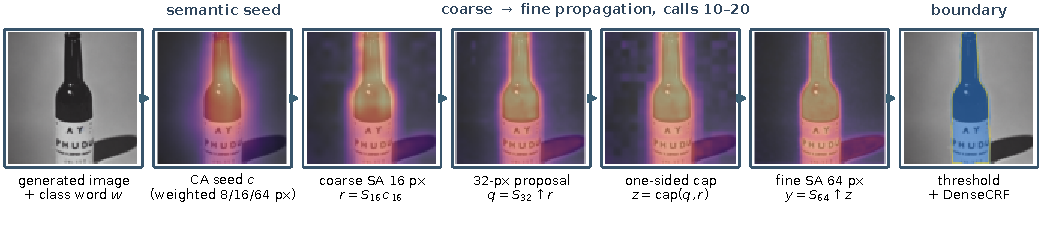
\includegraphics[width=\textwidth]{figures/method_overview.pdf}
\caption{\textbf{From semantic evidence to an object mask.} A class-word attribution prompt yields a CA seed; the selected 64-pixel SA module propagates that seed twice within each call--head observation; the observations are averaged and the fixed DenseCRF refines the thresholded map using RGB boundaries. We select settings on VOC-Sim folds and only then score COCO-Cap. The diagram describes the confirmed training-free path; the later middle-call variant changes only the SA observation set.}
\label{fig:overview}
\end{figure*}
